\documentclass[article.tex]{subfiles}
\begin{document}

\section{Case Study: Hexagonal surface panelization}
\label{sec:panelization}
Here we present the findings of a first case study, where the method
of discrete conformal mappings was utilized for a real-world project.
In this case study, a facade design, important questions concerning
panel layout, similarity and therewith constructability had to be
addressed at the early design stage.

Discrete conformal maps were used, as they allow the designer to
explore alternative surface textures and surface panelizations with
great design flexibility. This distinguishes the method from more
constrained modelling techniques~\cite{Ceccato}. Through the method of
conformal mapping, opposed to naive UV mapping, the density of the
surface panelization varies across the entire surface, yet the shape
of elements does not. This can be used for structural purposes, such
as diagrid layouts, or design driven, such as window distribution, see 
Figure~\ref{fig:entrance}. The optimization of the surface panelization 
towards multiple criteria such as edge length and planarity was 
consequential.

\begin{figure}[t]
  \centering
  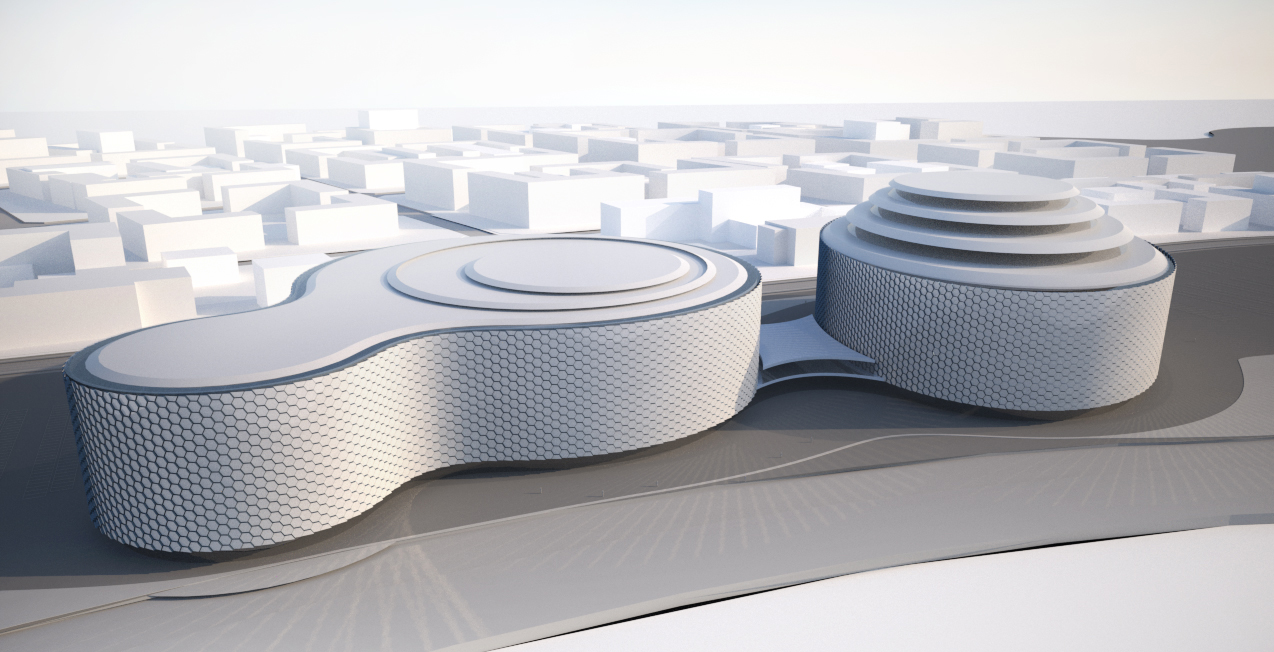
\includegraphics[width=0.93\textwidth]{images/henn/overview02.jpg}
  \caption{Rendering of Case Study - A project where the method of
    conformal mapping was utilized for the facade design.}
  \label{fig:overview02}
\end{figure}

For a commissioned competition entry we tested and developed the
method of periodic conformal mappings. The project, which served as a
case study, was highly constrained, as the architects were asked to
propose an alternative facade design for an existing design proposal
of a multifunctional exhibition center in China, see
Figure~\ref{fig:overview02}. The massing was fixed, but there were 2
alternative massing options (1 single curved and 1 doubly-curved
envelope) to be explored. Also, the client wanted a hexagonal tiling
on the facade but only had a very limited budget of approximately 200
Euro / sqm for the entire facade including sub structure in mind.

These limitations, in combination with the very short timeframe of 2
weeks for the entire redevelopment of the facade including a
feasibility study drove the development of the conformal mapping
method. Especially, since existing solutions such as UV mapping led to
unsatisfactory results producing anisotropic stretch and shear of some
regions in the master surfaces.  Some specific questions that had to
be addressed for each massing option were:
\smallskip
\begin{compactitem}
\item How many (different) panels would we need?
\item Can we clad the entire surface with planar tiles?
\item Can we equalize the edge lengths of each hexagon?
\item Can we control the orientation of the panels?
\item Can we achieve a regular pattern with a homogeneous visual
  appearance?
\end{compactitem}
\smallskip
In the end, all the above questions were answered/solved.

The first step of development focused on achieving periodicity across
the surface and alignment with the boundary. While the issue of
periodicity directly addressed the last question, it is strongly
related to the others as they could be achieved by successive
optimization steps.

\begin{figure}[t]
  \centering
  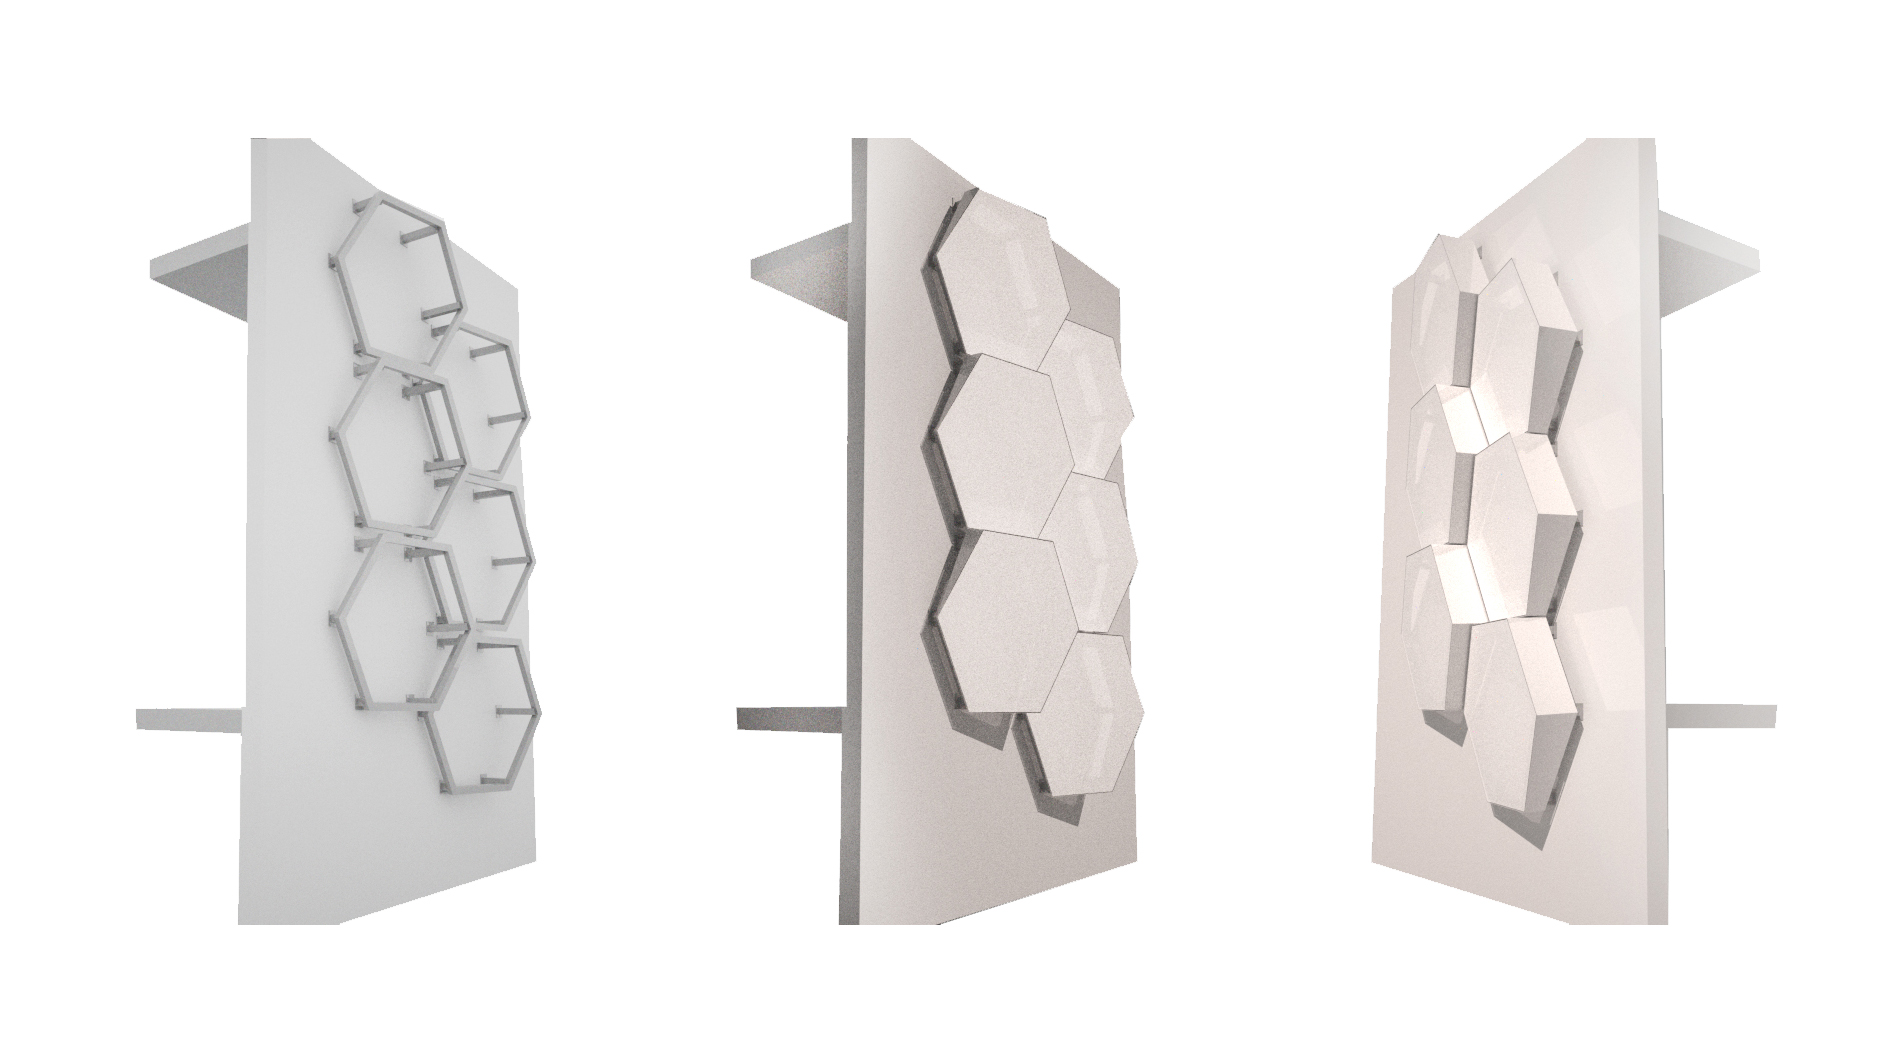
\includegraphics[width=0.93\textwidth]{images/henn/panel_construction.jpg}
  \caption{The data for the component-like construction of each panel was derived from the mesh.}
  \label{fig:panel_construction}
\end{figure}

Already during the design phase a fully periodic tiling was
achieved. In a following step the panels were planarized, grouped by
dimension and their edge lengths were equalized. Finally, a control
for the panel orientation based on the tangents of the \nurbs master
surface was implemented. This hexagonal pattern served as a base for
the facade engineering team. Due to the high cost demands, a simple
component system that served as a sub-structure for each panel was
developed, see Figure~\ref{fig:panel_construction}.

Unfortunately the given massing options for the building were not very
challenging in terms of geometry. One massing option was a simple
extrusion and the other had very little distortion. After the
successful submission of the project, we decided to continue the
development and test the method of discrete conformal mappings on more
extreme base geometries.

During these tests a Grasshopper plug-in for \VaryLab,
see~\cite{varylab-web-page} has been developed and refined. We focused
on tiling surfaces with a large distortion/stretch and double
curvature. The main aim was to tile these surfaces without
distorsion. This led to focus on the boundary conditions. The designer
is now able to choose between an aligned mapping where the tile-pattern
aligns with the underlying surface boundary. The trade-off being, that
panels need to vary in sizes. Or one chooses a ``homogeneous tiling'',
where all the tiles are the same, but do not align with the
boundary. \VaryLab's numerous optimization algorithms can be applied
and combined with either of the two approaches, see
Figure~\ref{fig:hex_example}. During the development, we realized that
through singularities and special boundary conditions, one is able to
control the density and distribution of the pattern on the surface and
along its boundaries, see Figure~\ref{fig:entrance}.

\begin{figure}[bt]
  \centering
  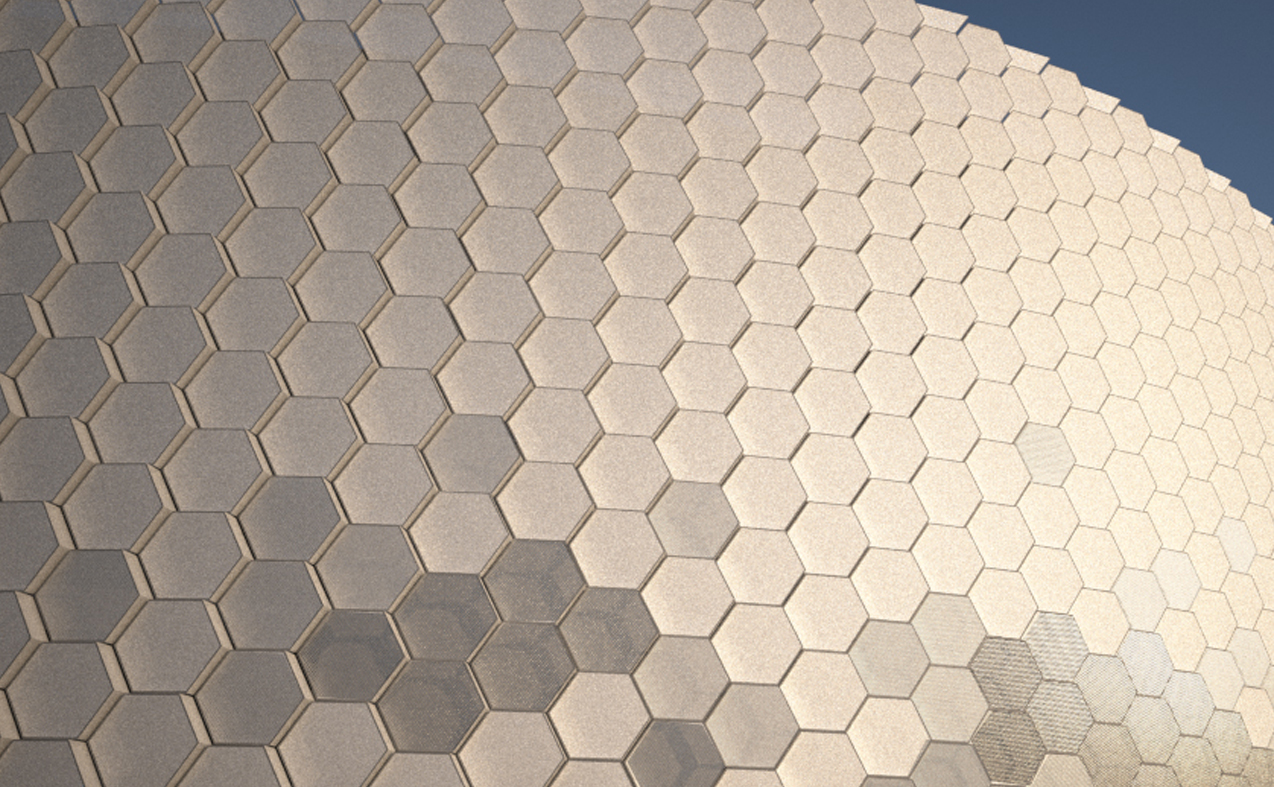
\includegraphics[width=0.93\textwidth]{images/henn/detail.jpg}
  \caption{Close-up rendering of facade.}
  \label{fig:detail}
\end{figure}

\end{document}

%%% Local Variables: 
%%% mode: latex
%%% TeX-master: "article"
%%% End: 
